% --------------------------------------------------------------
% This is all preamble stuff that you don't have to worry about.
% Head down to where it says "Start here"
% --------------------------------------------------------------

\documentclass[11pt]{scrartcl}

\usepackage{natbib}
\usepackage{geometry}
\usepackage{amsmath,amsthm,amssymb,url}
\usepackage{fullpage}
\usepackage{tabularx}
\usepackage{float}

\usepackage{graphicx}
\usepackage{xcolor}
\definecolor{darkblue}{rgb}{0,0,0.5} 
\usepackage{transparent}

\usepackage{enumitem}
\setlist{nolistsep}

\setlength{\parskip}{3px}

%\addtolength{\topmargin}{-.5in}
%\addtolength{\textheight}{1.2in}

\newcommand{\N}{\mathbb{N}}
\newcommand{\Z}{\mathbb{Z}}

\newenvironment{theorem}[2][Theorem]{\begin{trivlist}
\item[\hskip \labelsep {\bfseries #1}\hskip \labelsep {\bfseries #2.}]}{\end{trivlist}}
\newenvironment{lemma}[2][Lemma]{\begin{trivlist}
\item[\hskip \labelsep {\bfseries #1}\hskip \labelsep {\bfseries #2.}]}{\end{trivlist}}
\newenvironment{exercise}[2][Exercise]{\begin{trivlist}
\item[\hskip \labelsep {\bfseries #1}\hskip \labelsep {\bfseries #2.}]}{\end{trivlist}}
\newenvironment{problem}[2][Problem]{\begin{trivlist}
\item[\hskip \labelsep {\bfseries #1}\hskip \labelsep {\bfseries #2.}]}{\end{trivlist}}
\newenvironment{question}[2][Question]{\begin{trivlist}
\item[\hskip \labelsep {\bfseries #1}\hskip \labelsep {\bfseries #2.}]}{\end{trivlist}}
\newenvironment{corollary}[2][Corollary]{\begin{trivlist}
\item[\hskip \labelsep {\bfseries #1}\hskip \labelsep {\bfseries #2.}]}{\end{trivlist}}

\begin{document}

% --------------------------------------------------------------
%                         Start here
% --------------------------------------------------------------

\title{Visualizing Physical Query Execution in a Relational Distributed Big Data Management System}
\subtitle{Short Project Description \--- Distributed Systems}
\author{Shumo Chu and Dominik Moritz}
\date{}

\maketitle

\section{Introduction}

Myria is a distributed big data management system currently being developed in the database group. Myria aims towards building a distributed database platform to provide \emph{big data management and analytics as a service} primarily for scientific applications. Myria can run queries from languages that are equivalent to relational algebra with recursion. Queries are translated to physical query execution plans and then executed in the system. At the moment, the only measure for query execution is the overall running time. This limitation led to extended debugging sessions where we tried to understand why certain queries run for a long time. This process was often not very successful and is clearly not effective.

We are building a system to collect information about the query execution and visualize the data in a meaningful way that will allow us to efficiently debug and improve query execution.


\section{Background and goals}

This section describes how queries are executed in the Myria system and how our project will help us to understand the execution of physical query plans.

\subsection{Background}
\label{sec:background}

Database system need to transform user's high-level queries, eg. SQL, Datalog into a physical query plan for the execution. The physical query plan is the actual execution map of a database system. Usually it can be viewed as a \emph{DAG}, which consists of basic operators, such as \emph{JOIN}, \emph{GROUP BY}, \emph{SCAN}, \emph{APPLY} and relational tables. In distributed database systems, the introduction of the \emph{SHUFFLE} operator and data partitioning makes query plans more complicated.

\begin{figure}
 \begin{center}
     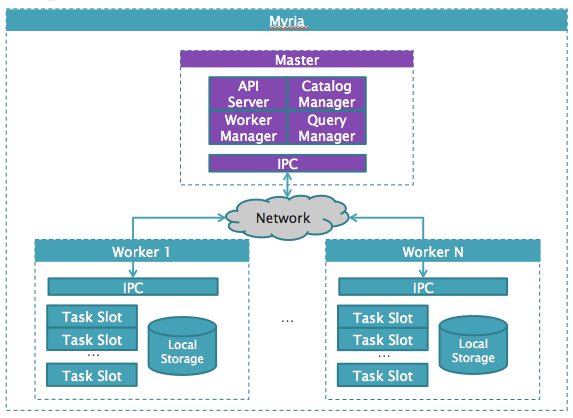
\includegraphics[width=0.7\textwidth]{myria.png}
   \end{center}
  \caption{distributed database architecture}
  \label{fig:myria_arc}
\end{figure}


\noindent\textbf{Distributed database system.} is a database system deployed on a cluster of servers. Figure~\ref{fig:myria_arc} shows the system architecture of the distributed database system we are working with. The master parses the query and distributes tasks to computing nodes (workers). The data is pre-partitioned and stored in the workers. Database queries in the form of SQL, Myrial\footnote{Myrial is a PigLatin like declarative language} or Datalog are translated to the physical query plan and then executed.

\noindent\textbf{Query Plan} is the actual execution map for the distributed database system.  Each query plan consists of basic operators forming an execution flow. For example, the SQL query $SELECT \; R.*, S.*  \; WHERE \; R.x=S.y ;$ can be translated to the visualized query plan shown in Figure~\ref{fig:query_plan}. The semantics of the query plan is a distributed hash join of two tables, $R$ and $S$. We first need to hash each table according to the joined fields. Then tuples are shuffled by their hash results to different workers. At each worker, the shuffled tuples are joined locally. A query fragment is a subtree of the query execution plan that is separated from the rest of the plan by a network boundary. The example has three query fragments. Each query fragment runs in a thread on each worker. Note that the query fragments do not form a DAG because of recursion.

\begin{figure}
 \begin{center}
     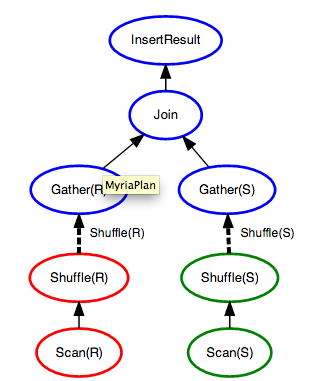
\includegraphics[width=0.35\textwidth]{partition_join.png}
   \end{center}
  \caption{Query plan: distributed hash join using three query fragments.}
  \label{fig:query_plan}
\end{figure}

\subsection{Goals}
\label{sec:objective}

% TODO: goals

Database system profiling has been extensively studied over decades. There are two types of works on this topic. One is logging query execution information and analyzing logs afterwards for better query optimization. The other is using real-time profiling information to estimate the progress of a query. We focus on the first type of problem in the context of distributed database system.

Tools to visualize query plans for example in SQL Server as used to improve performance for the SDSS Sky survey\cite{szalay2002sdss} focus on optimizing queries and not query execution and have no visualization of data flow which is necessary to optimize physical query execution.

Our system has to collect information about the execution of a physical query plan in Myria, which provides the foundation for analyzing the data and creating a meaningful visualization. The visualization will be embedded in a web application. We plan to analyze the query execution and find problems such as data skew.

\vspace{5px}

\noindent Questions that we want to answer with this project:

\begin{enumerate}
  \item What are the data dependencies between operators in workers?
  \item What is the bottleneck of the execution? Improving which part could improve the performance the most?
    %\item How does an optimization rule affect query execution?
  %\item Is an execution network or CPU bound?
  \item Is there a slow worker during a certain stage of the execution that prevent the progress of the whole query plan?
  \item Is the data skewed in a way that prevents efficient usage of available workers?
  \item How does network and computation contribute to the total running time? We make two hypothesis, respectively. If we assume the network has infinite bandwidth and no latency, how would the running time change? If we assume that we have infinite computation power, how would the running time change?
  %\item How good is the load balancing? If it is skewed, how much does this affect the performance?

\end{enumerate}


% explain what we want to learn about operators, query fragments and workers
% talk about shared memory model

\subsection{Design and implementation}

In Section~\ref{sec:logging}, we will describe how we collect performance data using logging and what the logs tell us about the query execution. In Section~\ref{sec:visualization}, we will focus on how we present this information to help us as developers to understand the performance impact of skew or certain operators on the running time. In Section~\ref{sec:overhead}, we will explain a method that we use to determine the communication and computation time of a query execution.

\subsubsection{Logging}
\label{sec:logging}

In our visualization, we want to capture the state of operators, query fragments, and workers. The state of a query fragment depends on the state of the operators inside it and the state of a worker depends on the state of the query fragments that are running on it. Consequently, we only need to capture the state of query fragments per worker. In order to capture state changes, we log events and state changes of operators. In the logs we look for events that indicate a state change. For each state we want to visualize when the transitions happened.

Not all operators have the same states. A consumer for example does not have a wait, compute or send state. Table~\ref{tbl:state} shows the different states operators can be in and briefly describes their meaning. Note that sleep and wait are different. Waiting means that an operator is waiting for child to return from a function call and sleep means that an operator has to be woken up by new incoming data.

\begin{table}[h]
\begin{tabularx}{\textwidth}{ l|X|X|X }
 & \multicolumn{3}{ c }{operator type} \\
\cline{2-4}
state & producers & consumers & operations \newline (\emph{JOIN}, \emph{MERGE}, \emph{SCAN}, \emph{APPLY}, ...) \\
\hline \hline
receive & - & receiving data from producer over network & - \\
\hline
wait & child is producing & - & waiting for child to return \\
\hline
compute & hashing data & - & in \texttt{fetchNextReady} and not waiting for any data \\
\hline
sleep & has data for consumer that is not ready & no data in producer & waiting for signal \\
\hline
send & sending data to consumer over network & - & - \\
\end{tabularx}
\caption{Possible states of operators and their meaning.}
\label{tbl:state}
\end{table}

In order to capture these states we have to log events that indicate their beginning and their end. An operator can only be in one state at a time. Consequently, the states can be reconstructed from the logs without any information about which events belong to each other. Since we also log the time of the events we can reconstruct when an operator changes its state and determine how long it has been in a certain state. We don't expect clock skew to be a problem because the intervals are coarse grained enough.

No all transitions between states are possible. For example, the wait state can only be reached from the compute state. A way to interpret this is that wait and compute are a sub-states of another state work. This interpretation is useful since a set of computes and waits can be grouped together because they were triggered by a call to \texttt{fetchNextReady} and end with a return from the function. We will use this information in the visualization of operator states.

To be able to reconstruct the states mentioned in Table~\ref{tbl:state} we have to log all events that cause state changes. Furthermore, we will log signals. % todo: do we actually need signals?

As mentioned in the beginning of this section, the states of query fragments and workers can be inferred from the state of the query fragments that are executed on a worker. A query fragment can be in the state receiving when the leave operator is a consumer (and not a scan). It can be in the state compute when any of its children are computing. It can be sleeping when the root is sleeping and it can be sending when the root is sending. Since a fragment is executed by one thread, it cannot be in multiple states.

The state of a worker is ambiguous because multiple threads can be executing multiple query fragments that are in different states. We will use the state of the query fragments to show how many query fragments are working but we will not determine a single state for the whole worker.

% state changes

For logging, we use standard Java logging using \emph{slf4j}\footnote{\url{http://www.slf4j.org}}, a logging API, which is implemented by different logging frameworks. Since logs are collected on different workers, we need to collect them on one machine that analyzes the data and creates the visualizations. The collecting server is a Myria worker, which means that we can use its database to store the logs and then read from when we create the visualization.

% how does the visualization server process the data

\subsubsection{Visualization}
\label{sec:visualization}
% Web client
% Form of visualization, e.g. what do we visualize, operator, query fragment, workers. In each kind of visualization, how will the interface looks like.
% What kind of information a potential user can get from the visualization.

At the moment, we support two views. One shows the state of one query fragment on each worker. The second view shows the states of one query fragment on one worker.

For the first view, we want to show on how many workers the query fragment is running at a certain point in time. To do this, we count the number and show a line plot as seen in Figure~\ref{fig:line}. This form of visualization was confirmed to be a good way to find data skew. Skew can be identified in a drop in the number of workers calculating a query fragment.

\begin{figure}[h]
  \begin{center}
    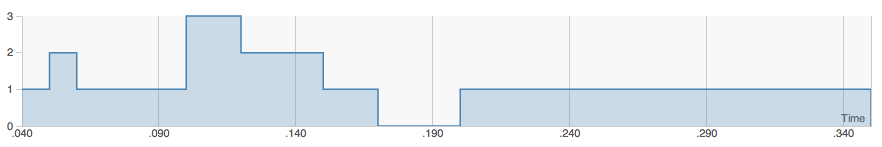
\includegraphics[width=1\textwidth]{line.png}
  \end{center}
  \caption{A line chart showing the number of workers on which a query fragment is running on.}
  \label{fig:line}
\end{figure}

We use a gantt chart to visualize the states and the times an operator or query fragment is in a state in the second view. Gantt charts are used widely in the visualization of project plans because they visualize time spans and show dependencies between them. For the visualization of operators we want to show the hierarchical relationship between operators and allow users to focus only on certain operators. Additional information about states (such as where the data is fetched from, specific parameters of an operator and eventually how much data was returned) will be shown on demand. Figure~\ref{fig:gantt} shows the visualization of operators in a query fragment.

The gantt chart is also used to visualize whether a query fragment on a worker is calculating or sleeping in addition to the plot in the first visualization. Instead of showing a hierarchy, only the states computing or sleeping are shown for the root operators of a query fragment on each worker.

\begin{figure}[h]
  \begin{center}
    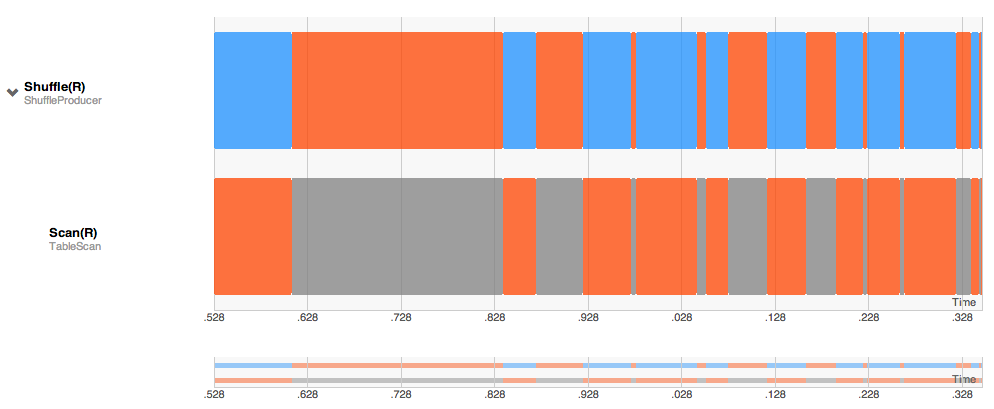
\includegraphics[width=0.9\textwidth]{realgantt}
  \end{center}
  \caption{Example gantt chart for a simple query fragment. Red is computing, blue is waiting and gray is sleeping. The small graph under the main graph allows users to select an area to focus on.}
  \label{fig:gantt}
\end{figure}

These kinds of visualization allow developers to answer the questions from Section~\ref{sec:objective} except for the last one. We will describe how we answer this question in Section~\ref{sec:overhead}.

For the final visualization, we plan to add another view that shows the graph that shows on how many workers a query fragment is running for each query fragment. The three views can be seen as showing different granularities. The overview over all query fragments reveals dependencies and a developer might want to investigate a certain query fragment that seems to block others. For this query fragment the developer can investigate its execution of different workers and potentially find the one that is slowing down the whole execution. Then the developer can evaluate why a particular query fragment on a worker is not working.

A more detailed evaluation of how the visualization helped us to understand, debug and eventually improve how queries are executed will be added in the final paper.

We use \emph{d3}\footnote{\url{http://d3js.org}} to build the visualization. D3 is a JavaScript framework for data visualizations on the web. Consequently, our visualization will be browser based and we integrated it into the existing web interface for Myria\footnote{A demo can be found at \url{http://myria-web.appspot.com} but it does not yet have the visualization.}.

%\subsubsection*{Analytics}
\subsubsection{Estimate computation/network overhead}
\label{sec:overhead}

A further question is  how can we get insightful information from the logging and visualization. To help us improving query plan rewriting and efficiently allocate resource for a query, we might want to reason about what factor contribute most to the running time of the query plan from the logging/visualization. In a pipelined and asynchronous query execution, since communication (via network) and computation are overlapped. There would be no accurate measure of the communication time and computation time for the whole system.  So we would like to ask following questions.

\noindent\textbf{Assume no communication time}.  That is to assume that we can have an underlying network with infinite bandwidth and zero latency. Based on the logging, we want to infer how much the running time could be improved given this assumption. This would be a measure of how expensive the computation is and could demonstrate the best performance gain we can have if we make the communication faster.

\noindent\textbf{Assume no computation time}.  That is to assume that we can have infinitely fast computation hardware. Given this assumption, we want to infer how much the running time could be improved. This would be a measure of how expensive the communication is.

\noindent\textbf{Proposed solution}.  Based on the logging information, we can build a temporal state transition graph of the query execution. This graph will consist of the temporal state information of each query fragment in each worker. Combined with the query plan which contains the dependency between different operators, we want to develop algorithms to infer the running time given different assumptions.
%\section{Result}
%\section{Summary}

%\section{Outlook}
%\label{sec:outlook}

\bibliographystyle{plain}
\bibliography{references}

\end{document}